\newpage

\section{Practical exercises}

\subsection{Disk usage visualization}

The \href{https://man.archlinux.org/man/du.1}{du} command can be used to
estimate the disk utilization of a file, or recursively scan a directory. When
using this command, you need to note that it does not differentiate between
cohesive files and \href{https://wiki.archlinux.org/title/Sparse_file}{sparse
files}. Additionally, \href{https://linuxhandbook.com/hard-link/}{hard links}
can trick you into thinking that your disk utilization can exceed the actual
storage space.

These are a few caveats that you would normally need to keep in mind, but for
this task we are going to focus on the plotting aspect. Go in your home
directory and use \texttt{du} recursively (see the \texttt{-s} flag) on all
subdirectories, but also any files residing directly in your home. Output their
size in bytes instead of kilobytes, then use the
\href{https://man.archlinux.org/man/sort.1}{sort} command to sort the items in
reverse numerical order, based on size (meaning largest first).

Write a Python script that takes this as input and generates a
\href{https://pythonguides.com/matplotlib-plot-bar-chart/}{bar plot}
illustrating how much space each file and subdirectory in your home takes up.

\subsection{CPU usage visualization}

As you know, your CPU has multiple cores. To find out exactly how many, you can
run the \href{https://man.archlinux.org/man/nproc.1}{nproc} command. In this
task we are going to run CPU intensive workloads on \textit{specific} cores and
create a bar plot representing the percentage of time each core spent executing
user level code (i.e., applications), system level code (i.e., kernel tasks
unrelated to servicing hardware peripherals) and hardware interrupts.

To gather this data, you can use the
\href{https://man.archlinux.org/man/mpstat.1}{mpstat} command. To
perform CPU-intensive work, take a look at the
\href{https://man.archlinux.org/man/stress.1}{stress} command. If left as it is,
the kernel's scheduler will most likely bounce the \texttt{stress} process from
one CPU core to another. Try using the
\href{https://man.archlinux.org/man/taskset.1}{taskset} command to bind multiple
\texttt{stress} workers to \textit{odd} CPU cores.

\subsection{Dynamic plotting}

Make sure that you have completed the previous task before starting this one.

\texttt{mpstat} can either report momentary statistics or it can do so
periodically. Try alternating the CPU load between even and odd cores on your
processor (see \href{https://man.archlinux.org/man/timeout.1}{timeout} and
\href{https://man.archlinux.org/man/sleep.1}{sleep}) and visualize these
statistics with a
\href{https://holypython.com/python-visualization-tutorial/creating-bar-chart-animations/}
{dynamic bar plot}.

\subsection{Pandas introduction}

Pandas is a Python library used in data manipulation and analysis. It is based
on \texttt{numpy} but introduces certain data structures such as
\href{https://pandas.pydata.org/pandas-docs/stable/reference/api/pandas.DataFrame.html}
{DataFrames} for managing tabular data, or
\href{https://pandas.pydata.org/pandas-docs/stable/reference/api/pandas.Series.html}
{Series} for handling 1D arrays (especially time series). Pandas also offers
tools for interacting with different storage formats such as CSV, Excel, SQL
databases, etc.

We recommend going over the official
\href{https://pandas.pydata.org/pandas-docs/stable/user_guide/10min.html}{10
minutes to pandas} crash course and keeping this
\href{https://github.com/pandas-dev/pandas/blob/main/doc/cheatsheet/Pandas_Cheat_Sheet.pdf}
{cheat sheet} at hand. Note that Pandas also has built-in plotting support,
even though it's based on \texttt{matplotlib}. See the
\href{https://pandas.pydata.org/pandas-docs/stable/user_guide/visualization.html}
{chart visualization} chapter in the official documentation and also look at
the \href{https://pandas.pydata.org/pandas-docs/stable/user_guide/cookbook.html#cookbook-plotting}
{cookbook} chapter for practical examples.

Try downloading \href{https://www.kaggle.com/datasets/themlphdstudent/countries-population-from-1955-to-2020}
{this kaggle dataset} containing per-country population statistics between
1955 and 2020 and plotting the demographic changes that can be extracted from
this data. Start with your own country and then perform a comparison with
immediate neighbours.

\subsection{Radio spectrogram}

In the assets directory, we have a \texttt{iq\_sample.raw} file containing
measurements of the FM radio spectrum performed with a
\href{https://blinry.org/50-things-with-sdr/}{Software Defined Radio (SDR)}. In
this exercise we are going to process these samples and obtain a spectrogram,
showing how the radio signal frequency changes in time.

\begin{figure}[h]
    \centering
    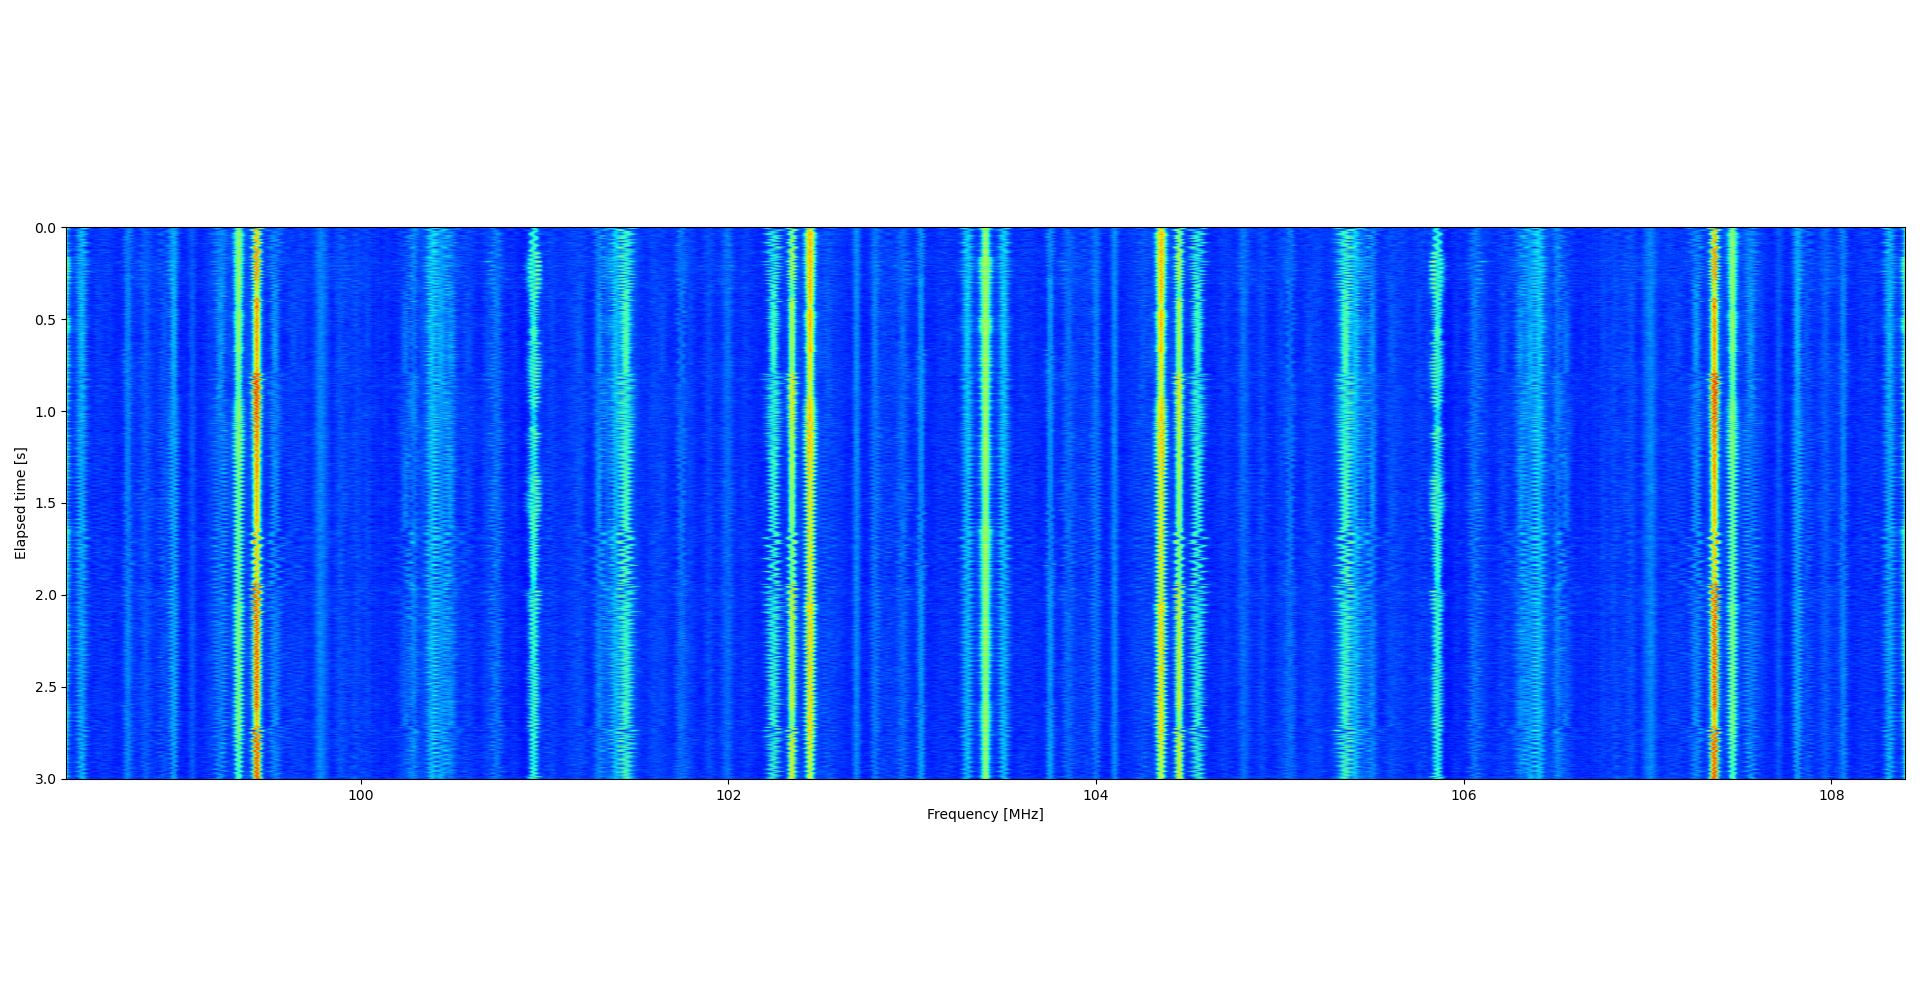
\includegraphics[width=\textwidth,keepaspectratio]{figures/waterfall.png}
    \caption{Spectrogram of radio signal.}
    \label{fig:spectrogram}
\end{figure}

In Figure \ref{fig:spectrogram} we see what is called a waterfall plot. The
signal that we recorded is comprised of multiple signals of \textit{specific}
frequencies. Each line of pixels represents the amount of power each individual
component exhibits in a limited timeframe. This information is encoded through
the pixel color, that adheres to the
\href{https://www.mathworks.com/help/matlab/ref/jet.html}{jet colormap} (i.e.,
blue is weaker, red is stronger). In this plot we notice that there are a few
frequency bands that consistently present high levels of power. These are
different radio stations. The small shifts in power distribution around these
frequencies over time is how sound is encoded when transmitted to our radio
devices.

\subsubsection{Parsing input data}

In order to acquire this data, we used a
\href{https://www.nuand.com/product/bladerf-xa9/}{bladeRF 2.0 micro xA9} SDR
and \href{https://www.gqrx.dk/}{GQRX} for data visualization and acquisition on
our host. We tuned our SDR to a frequency of 103.4MHz and used a sampling rate
of 10MHz. The sampling rate determines how wide the frequency spectrum that
we visualize can be. In this case, the Ox axis of our previous figure is defined
between 103.4 ± 5MHz.

SDRs usually work with complex sampling, also known as
\href{https://pysdr.org/content/sampling.html}{In-phase Quadrature (I/Q)
sampling}. Instead of providing a real value representing the amplitude of the
signal at a given time, this technique provides a number of benefits. These are
not relevant to the exercise at hand but just to get an idea, if we were working
with \textit{real} numbers instead of \textit{complex} numbers, we wouldn't be
able to "see" frequencies at ±5MHz around our tuned radio frequency. Instead,
we would only be able to see the positive half of the spectrum.

Our particular SDR provides 4 bytes for each I/Q sample. The first two bytes
represent the real component and the last two bytes represent the imaginary
part. Each of these two bytes must be interpreted as \textbf{unsigned short}
values. A value of 0x0000 represents the \textit{minimum} value that the SDR
can record and 0xffff represents the \textit{maximum} value. The exact values
do not necessarily interest us since we only want to observe differences between
the presence and the lack of a signal. Information about the range of measurable
values can be found in the data sheet of the SDR.

To start things off, read the data from the provided \textbf{binary file} and
use the \texttt{struct} module to \textbf{unpack} the data into unsigned shorts.
Create an array of \textbf{complex} values representing our samples. Note that
python has built-in support for complex number representation (e.g.,
\texttt{1 + 2j}).

\vskip .5cm

\textbf{Tip \#1:} The sampling frequency that we used might have been a bit too
high, resulting in a large amount of data. If you notice that you are running
low on RAM while solving this exercise, consider employing
\href{https://dspguru.com/dsp/faqs/multirate/decimation/}{signal decimation}.
Effectively, you can select only every second, or fourth, or eighth, etc.
sample. This will reduce the memory consumption but the width of the frequency
spectrum will also be reduced by a factor of 2, 4, 8, and so on.

\textbf{Tip \#2:} When you are done with certain data stored in a variable
\textbf{x} let's say, consider running \textbf{del(x)} to free up the memory.
For this subtask, you may load the raw I/Q sample file in memory and then
process it into an array of complex numbers. If the array is stored in a
different variable than the raw data, the garbage collector will not free up
the raw data buffer since there is still a reference to it.

\subsubsection{Convert to frequency domain}

Now that we have an array of I/Q samples, we can convert the signal from the
time domain to the frequency domain. This can be done using the
\href{https://numpy.org/doc/2.1/reference/generated/numpy.fft.fft.html#numpy.fft.fft}
{Fast Fourier Transform (FFT)}. The FFT takes a time series of complex numbers
and outputs yet another series of complex numbers, but this new series will
be in the frequency domain. The range of frequencies is determined
\textit{solely} by the tuned frequency (103.4MHz) and the sampling frequency
(10MHz if not decimated).

At this point, we could compute the FFT on the entirety of our sampled signal.
However, this will only show us the amount of power dissipated for each frequency
during the entire lifetime of the signal (or rather, our measurement). In other
words, we would not be able to see the \textit{evolution in time}. The solution
is simple. We must create a \textit{sliding window}; a continuous subset of
samples on which we apply the FFT. By shifting the window to the right, we
advance in time but maintain a limited scope for our frequency analysis. The
result of this operation will be an array of FFT outputs, each representing a
\textbf{line} in our final plot.

\vskip .5cm

\textbf{Tip \#1:} Try to pick a power of 2 as the size of the window. This helps
optimize the computation of the FFT.

\textbf{Tip \#2:} It is your choice by how much you wish to advance the sliding
window. Yes, you can have overlaps between consecutive snapshots. Just note that
the smaller you step is, the longer it will take to finish the computation.
More lines, means more FFT function calls (which are expensive), means more time
spent prototyping. Consider using a step value equal to the size of the window.

\textbf{Tip \#3:} When choosing the FFT window size, remember that this will
\textbf{not} affect the frequency visibility range. It will still be 103.4 ±
5MHz regardless of your choice. What will be affected however is the precision.
If you compute a FFT on a small number of samples, let's say 100, then the range
of frequencies that is determined by the sampling frequency (i.e., 10MHz) will
be split into 100 "buckets" of 100kHz each. If two or more \textit{distinct}
signals fall withing the same "bucket", they will be represented as a single
signal. If you decide to use 10,000 samples instead, you will have 1kHz buckets
instead of 100kHz buckets, which may be enough for you to distinguish the two
signals.

\subsubsection{Post processing}

Now that we have one complex value for each pixel that we should render, the
question is how do we visualize this data? First of all, we need to convert each
complex number to a real domain value by computing its magnitude. Yes, there is
a function for this in the \texttt{numpy} module.

While computing the magnitudes, our suggestion is to also compute the natural
logarithm of these values. In signal processing the decibel (dB) scale is
commonly used in order to represent relative differences in power or amplitude,
which are more significant than absolute differences. This is also why we did
not bother to look up what the I and Q component value range is, at the start of
this exercise. Additionally, using a logarithmic scale can help emphasize lower
frequencies. This is especially helpful in speech recognition but it also
severs to highlight certain features in this example.

\vskip .5cm

\textbf{Tip \#1:} Note that the result may be noisy. In this case, you could
perform a \href{https://en.wikipedia.org/wiki/Moving_average}{moving average}
over each line to smooth out the data. The process is similar to the sliding
window FFT computation, but with a few notable distinctions. First, we are going
to be using the
\href{https://numpy.org/doc/stable/reference/generated/numpy.average.html}{
average} function instead of the FFT. Second, when computing a moving average
it is best to have a small step relative to the window size. Having a high
overlap between consecutive windows helps maintain the cohesion of the data that
we want to display. Finally, the window size itself should be as small as
possible. If it's too large, we will eliminate relevant features from our data.
However, if it's too small, the result will still contain noise. Start off with
a value of 30 and see what works.

\subsubsection{Plotting}

Finally, use the
\href{https://matplotlib.org/stable/api/_as_gen/matplotlib.pyplot.imshow.html}{
imshow} function from \texttt{pyplot} to plot the data. The \texttt{cmap}
argument can be used to select the color grading for the heatmap. In our example
use used \texttt{jet} but there are
\href{https://matplotlib.org/stable/users/explain/colors/colormaps.html} many
alternatives. Also, use the \texttt{extent} argument to set the numeric ranges
for the Ox and Oy axes. We've already mentioned what the frequency range is.
The elapsed time for the signal measurement can be computed based on the number
of samples and the sampling frequency.

